\chapter{Temperature and Emissivity Separation}
\label{chap:TES}

Pre-processed thermal image data provide valuable information about the properties of the observed surfaces, most importantly their temperature and emissivity. But in order to determine temperature and emissivity from observed radiance one must solve system of RTEs. Data from multispectral and hyperspectral TIR sensors offer the opportunity to derive both the temperature as well as an emissivity spectrum, which can be used to characterize the material composition of surfaces. However, observing radiance in $N$ bands yields $N$ RTEs but $N+1$ unknowns ($N$ emissivities plus temperature), which results in the underdetermined system of equations. The estimation of temperature and emissivity from such a system of equations is usually addressed as \textit{temperature-emissivity separation}. This chapter describes several approaches for separating temperature and emissivity. It firstly introduces few commonly used ones and then focuses on the most popular approach called Temperature and emissivity separation algorithm (TES). Last part of this chapter focuses on enhancing the accuracy and precision of the products generated by the TES algorithm. The main improvement is accomplished by replacing one of the TES modules with a newly designed one that takes advantage of a relationship between brightness temperature and emissivity. The improved TES algorithm is called Optimized Smoothing for Temperature Emissivity Separation (OSTES).

\section{Available approaches}

Many approaches have been developed to overcome the problem of having an underdetermined system of RTEs \cite{LT13}. Methods used to overcome the problem of underdetermined system of RTEs are usually based on adding empirical or semiempricial constraints. 

Algorithms for temperature and emissivity estimation depend on sensor architecture and acquisition context. Some algorithms require knowledge of Normalized Difference Vegetation Index (NDVI) \cite{SR00}, surface type \cite{SW98} or even emissivity \cite{JC09}. Others are based on multitemporal \cite{W08} or multiangle \cite{SS07} acquisition. There are only a small number of algorithms for simultaneous temperature and emissivity retrievals from a single scene without ancillary surface information, that are robust enough to be applicable to data acquired by multispectral or hyperspectral sensors. The most common are: grey body emissivity method \cite{BP96}, linear emissivity constraint temperature emissivity separation method \cite{WW11}, spectral smoothing \cite{B08} and the TES algorithm \cite{GR98}. Principles of last four mentioned methods are described in the following text. The most attention is paid to the TES algorithm, as it is the most popular and it is widely applied to many sensors.

\subsection*{Gray body emissivity method}

Barducci and Pippi \cite{BP96} proposed algorithm, which is based on assumption of flat spectral emissivity beyond $\SI{10}{\micro\meter}$. To solve the system of RTEs it is enough to find at least two spectral bands with the same emissivity. This can be achieved in case of airborne thermal hyperspectral data. Drawback of this method is its sensitivity to instrument noise.

\subsection*{Linear emissivity constraint temperature emissivity separation method}

As Wang et al. \cite{WW11} describe, this method is based on idea of substituting spectral emissivity with piecewise linear function. The emissivity spectrum is divided into segments, in which spectral emissivities are assumed to be linearly dependent on wavelength. Thus, it is necessary for every segment to estimate gain and offset. It implies that the number of spectral bands has to be equal or greater than number of unknowns resulting from segmentation to piecewise linear functions.

\subsection*{Spectral smoothing}

Spectral smoothing algorithm, also known as ARTEMISS (Automatic Retrieval of Temperature and EMIssivity using Spectral Smoothness), was reported by Borel at \cite{B98} and \cite{B08}. Algorithm is based on the assumption that spectra of solids are much more smoother than spectra of gases. Thus by smoothing spectra one removes spectral features introduced by atmosphere and obtains spectral emissivity. Moreover, current implementation described in \cite{B08} includes modified ISAC algorithm called ARTISAC, which estimates atmospheric transmissivity for further choice correct atmospheric model. Atmospheric models contains so called TUD (atmospheric Transmissivity, Upwelling and Downwelling atmospheric radiance) and are stored in look-up tables (LUT). Then temperature is varied until the spectral emissivity is the smoothest possible, where the smoothness criterion is standard deviation of measured radiance minus simulated radiance. Spectral smoothness method can be described briefly by following steps:
\begin{enumerate}
	\item estimation atmospheric transmissivity using ARTISAC algorithm
	\item determination few closest atmosphere models from TUD-LUT according to the estimated atmospheric transmissivity
	\item use these atmosphere models as input to spectral smoothness algorithm for a few pixels chosen from the image and the atmosphere model which results in smoothest emissivity in the most of the cases is chosen as the correct one
	\item use chosen atmosphere model for the whole image and estimate temperature and emissivity by applying spectral smoothing procedure
\end{enumerate}

\section{Temperature and emissivity separation algorithm (TES)}

TES algorithm was originally developed for the Advanced Spaceborne Thermal Emission and Reflection Radiometer (ASTER) sensor \cite{GR98}. ASTER was launched in December 1999 onboard NASA's Terra platform. TES has since then found widespread use with other multispectral and hyperspectral sensors. Several studies have discussed the implementation of TES with Airborne Hyperspectral Scanner (AHS) data \cite{SJ06, JS12}. Application of TES to data acquired by the TASI sensor is mentioned in a few studies as well \cite{WX11, PP12}. Apart from the mentioned sensors, the TES algorithm has been modified for the Digital Airborne Imaging Spectrometer (DAIS) sensor \cite{SJ02}. Concerning spaceborne sensors, the TES algorithm has also been suggested for Spinning Enhanced Visible and Infrared Imager (SEVIRI) \cite{JS14}, Moderate Resolution Imaging Spectroradiometer (MODIS) \cite{HH11} and Multispectral Thermal Imager (MTI) \cite{MB02} data processing. Moreover, the TES algorithm is being suggested for the future HyspIRI mission \cite{HH11-2}.

The TES algorithm is based on a semi-empirical relationship between spectral contrast (i.e. difference between the highest and lowest values in the emissivity spectrum) and the minimum emissivity. The algorithm consists of three modules, namely the Normalization Emissivity Module (NEM) \cite{G86}, the Ratio module and the Maximum-Minimum Difference (MMD) module \cite{M94}. The inputs of the algorithm are land-leaving radiance $L_\mathrm{LL}$ and downwelling radiance $L^{\downarrow}_\mathrm{atm}$. Let us remind the reader that land-leaving radiance is obtained from (\ref{eq:RTE}) by compensating for atmospheric transmissivity $\tau$ and atmospheric upwelling radiance $L^{\uparrow}_\mathrm{atm}$:
\begin{equation}
\label{eq:landleavingRadiance}
L_\mathrm{LL} = \varepsilon B(T_\mathrm{s}) + (1 - \varepsilon) L^\downarrow_\mathrm{atm}.
\end{equation}

The NEM module performs an iterative process for estimating temperature and emissivity, and compensating for the downwelling radiance. The output of the NEM module is an initial estimation of temperature and emissivity. Then the ratio module normalizes the emissivities obtained by the NEM module by their arithmetic mean. Thus one obtains the so called $\beta$ spectrum, which should be less sensitive to sensor noise. Finally, the maximum and minimum of the $\beta$ spectrum are found and their difference (MMD) is used in following semi-empirical relationship:
\begin{equation} 
\label{eq:MMD}
\varepsilon_\mathrm{min} = 0.994 - 0.687 \times \mathrm{MMD}^{0.737}. 
\end{equation}
Derivation of (\ref{eq:MMD}) is explained in following paragraph. Ratioing the $\beta$ spectrum back to an emissivity spectrum with knowledge of minimum emissivity results in a more precise estimation of the emissivity spectrum. The band with highest emissivity is then used for temperature estimation.

\begin{figure}[!t]
	\centering
	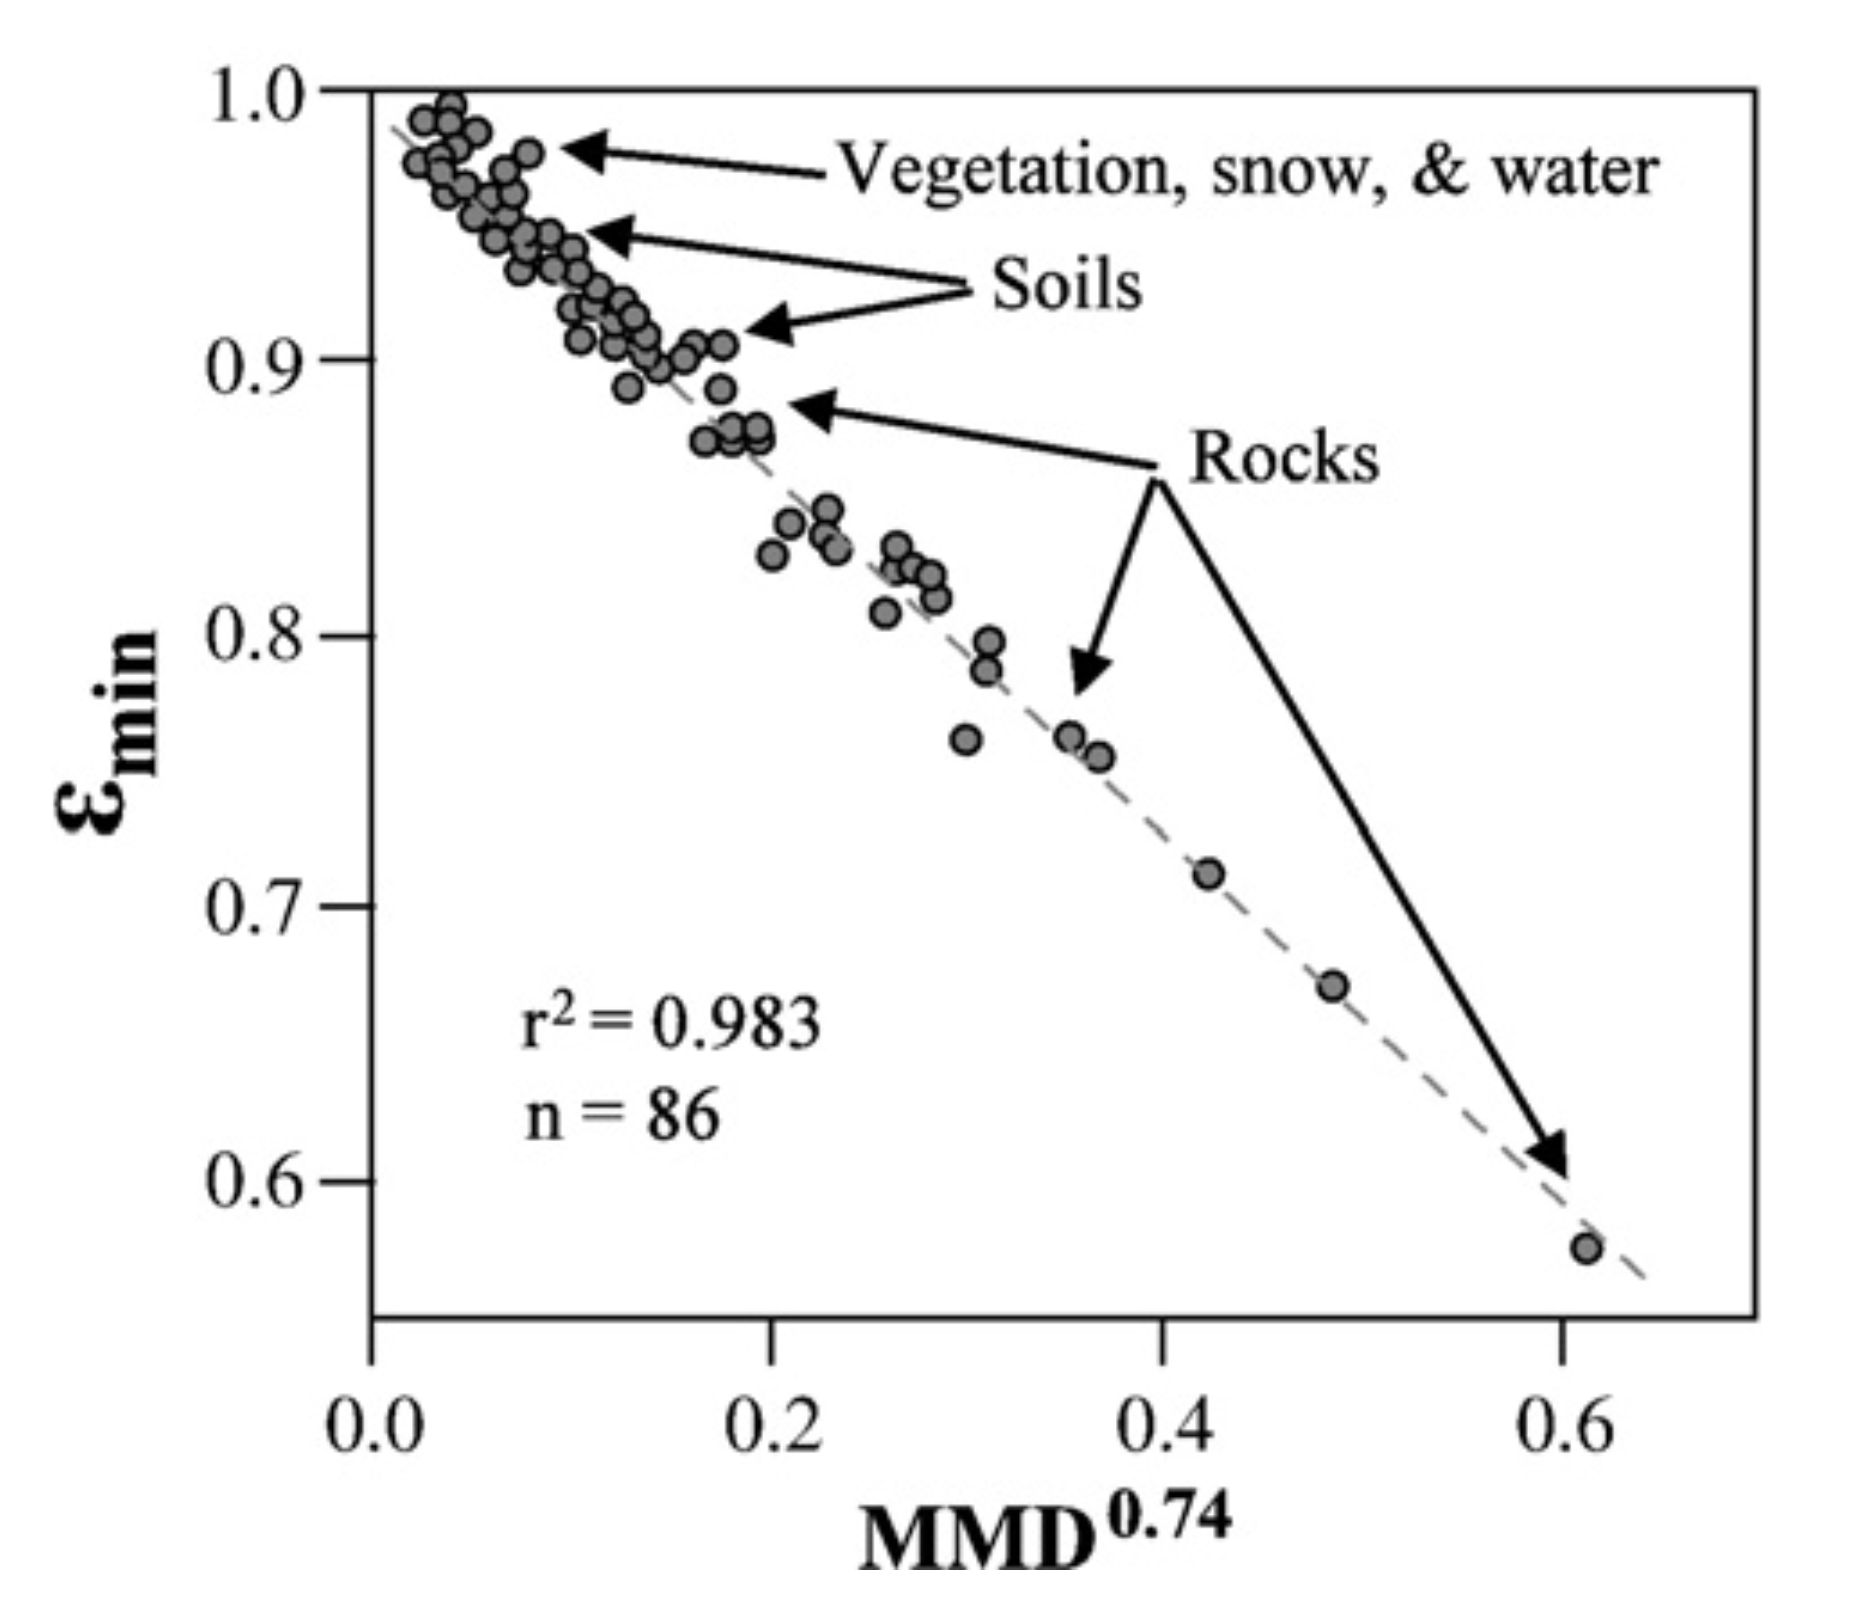
\includegraphics[scale=0.2]{pics/Chapter_03/EpsMinMMD.png}
	\vspace{1.5 em}
	\caption{Semi-empirical relationship between emissivity contrast and minimum spectral emissivity as shown in study reported by Sabol et al. \cite{SG09}.}
	\label{fig:EpsMinMMD}
\end{figure}

The relationship between spectral contrast and minimum emissivity, shown in (\ref{eq:MMD}), is a regression based on 86 laboratory spectra of rocks, soils, vegetation, snow and water chosen from the ASTER spectral library \cite{BH09}. This relationship is depicted in the Figure \ref{fig:EpsMinMMD}. It is important to note that (\ref{eq:MMD}) is tailored for the ASTER sensor. To apply  {TES to a} different sensor,  {the} regression of $\varepsilon_\mathrm{min}$ on MMD  {must be} refined by using sensor specific response functions. 

After ASTER was launched, \cite{GG06} and \cite{SG09} suggested to replace the power regression shown in (\ref{eq:MMD}) with linear regression. The replacement is connected with modification of the threshold for separating materials with low spectral contrast. The main advantage is elimination of artefacts in retrievals. However, the drawback is loss of accuracy in cases of materials with low spectral contrast \cite{SG09}. The TES algorithm used for generation ASTER standard products \cite{B15}, as well as its modifications for other sensors \cite{SJ06, JS12, WX11, SJ02, JS14, HH11, MB02, HH11-2}, is based on the power law regression. Thus, in this work the TES algorithm is considered to be that using the power regression.

\section{TES Algorithm Improvement}

The algorithm described below brings a new approach for the TES algorithm by replacing the NEM module with a completely new module. The new module is based on the similarity between brightness temperature spectral features and emissivity spectral features. Brightness temperature is obtained from land-leaving radiance under the assumption of emissivity $\varepsilon=1$ for every wavelength. Although land-leaving radiance includes some portion of reflected downwelling radiance, it still retains the spectral features arising from the emissivity of the surface materials, which is $0.6$ or higher for natural materials \cite{GR98}. Since the magnitude of downwelling radiance is usually much lower than the surface radiance the features contained in the brightness temperature spectra may be distorted but will not be completely hidden. The new module approximates this relation between brightness temperature $T_\mathrm{b}$ and emissivity.

\begin{figure}[!t]
	\centering
	\vspace{1em}
	\begin{subfigure}[t]{.3\linewidth}
		\centering
		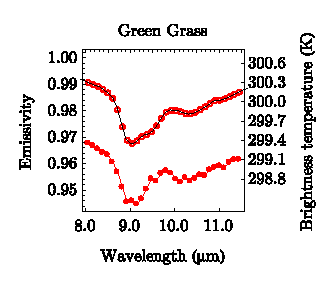
\includegraphics[scale=1]{pics/Chapter_03/GreenGrass_Emiss_vs_BrightTemp.eps}
		\caption{}
	\end{subfigure}
	\hspace{1em}
	\begin{subfigure}[t]{.3\linewidth}
		\centering
		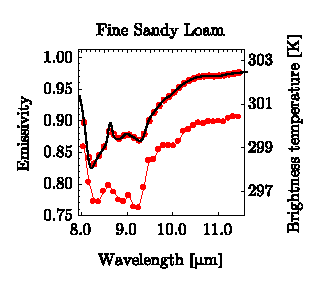
\includegraphics[scale=1]{pics/Chapter_03/FineSandyLoam_Emiss_vs_BrightTemp.eps}
		\caption{}
	\end{subfigure}
	\hspace{1em}
	\begin{subfigure}[t]{.3\linewidth}
		\centering
		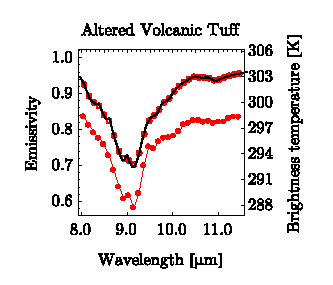
\includegraphics[scale=1]{pics/Chapter_03/AlteredVolcanicTuff_Emiss_vs_BrightTemp.eps}
		\caption{}
	\end{subfigure}
	\vspace{1.5 em}
	\caption{Emissivity spectra (black solid line) of three samples chosen from ASTER spectral library \cite{BH09}. Symbols represent band-effective values of emissivity (empty symbols) and brightness temperature (full symbols) for TASI sensor. }
	\label{fig:emissivitySpectra_spectra}
\end{figure}

In order to demonstrate the relationship, three emissivity samples with different spectral contrasts were chosen from the ASTER spectral library \cite{BH09}, namely green grass, fine sandy loam and altered volcanic tuff. Emissivities are depicted in Figure \ref{fig:emissivitySpectra_spectra} (solid lines) together with corresponding band-effective values for TASI sensor (empty symbols). These emissivities were applied to Plank's law at temperature $300\,\mathrm{K}$ and combined with downwelling radiance from standard mid-latitude summer atmosphere generated by MODerate resolution atmospheric TRANsmission (MODTRAN) \cite{BG06}. The resulting radiances, were transformed to band-effective quantities with respect to TASI response functions. Brightness temperatures for every band of each sensor were obtained by applying inverse Planck's law on sample land-leaving radiances under the assumption of $\varepsilon=1$. Figure \ref{fig:emissivitySpectra_spectra} also includes brightness temperatures (full symbols) in order to demonstrate spectral similarity with emissivity. Figure \ref{fig:relationship} plots emissivity against brightness temperature for chosen samples (empty symbols). These quantities clearly exhibit relationship with linear trend regardless of spectral contrast. Figure \ref{fig:relationship} also displays lines that approximate this relationship, derived in the manner described later in the next. The algorithm description below uses band-effective values of quantities linked to $i$-th band by subscript index $i$. 

Spectral features of brightness temperature will be further used for emissivity estimation. The dependence of emissivity $ {\varepsilon_i}$ on brightness temperature $ {T_{\mathrm{b}_i}}$ will be approximated by following equation:
\begin{equation} \varepsilon_{ {i}} =  {p} T_{\mathrm{b}_{ {i}}} +  {q}, \label{eq:relationship}\end{equation}
where $ {p}$ and $ {q}$ are empirical coefficients. These coefficients are determined by solving the system of two equations using two points, namely maximum brightness temperature coupled with emissivity equal to 1 and minimum brightness temperature coupled with lowest emissivity $\varepsilon_\mathrm{min}$:
\begin{equation}
\begin{aligned}
	1 &=  {p} \max (T_{\mathrm{b}_{ {i}}}) +  {q}, \\
	\varepsilon_\mathrm{min} &=  {p} \min (T_{\mathrm{b}_{ {i}}}) +  {q}.
\end{aligned}
\label{eq:sytemofeq}
\end{equation}
The next step is estimation of the the lowest emissivity $\varepsilon_\mathrm{min}$.

This is done by varying $\varepsilon_\mathrm{min}$ over the range  {of possible emissivities for natural materials $[0.6,1{ {]}}$}, determining corresponding coefficients $ {p}$ and $ {q}$ by solving (\ref{eq:sytemofeq}) and then approximating emissivity by (\ref{eq:relationship}) using brightness temperature for all spectral bands. The estimated emissivity is then used together with land-leaving radiance $L_\mathrm{LL}$ and downwelling radiance $L^\downarrow$ in a computation that yields spectral radiance:
\begin{equation}
	L^{\prime}_{ {i}} = \frac{L_{\mathrm{LL}_{ {i}}}-(1-\varepsilon_{ {i}})L^\downarrow_{ {i}}}{\varepsilon_{ {i}}}.
	\label{eq:lprime}
\end{equation}
The temperature in every spectral band is derived from spectral radiance $L^{\prime}$ applying inverse Plank's law. The highest one is chosen as the reference temperature $T_\mathrm{max}$. Finally, the estimated spectral radiance $L^{\prime}$ and Planck's law at the reference temperature $T_\mathrm{max}$ are normalized and compared against each other as follows:
\begin{equation*}
	\sum_{ {i}} \left| \frac{B_{ {i}}(T_\mathrm{max})}{||B(T_\mathrm{max})||_1} - \frac{L^\prime_{ {i}}}{||L^\prime||_1} \right|.
\end{equation*}
The value of $\varepsilon_\mathrm{min}$ is considered final if its corresponding spectral radiance $L^{\prime}$  {is the best fit to Plank's law}.

\begin{figure}[!t]
	\centering
	\vspace{1em}
	\begin{subfigure}[t]{.3\linewidth}
		\centering
		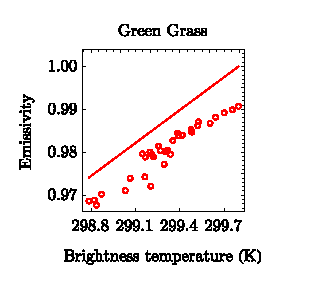
\includegraphics[scale=1]{pics/Chapter_03/GreenGrass_Emiss2BrightTemp.eps}
		\caption{}
	\end{subfigure}
	\hspace{1em}
	\begin{subfigure}[t]{.3\linewidth}
		\centering
		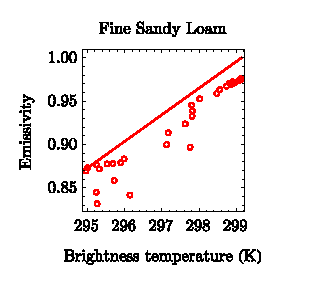
\includegraphics[scale=1]{pics/Chapter_03/FineSandyLoam_Emiss2BrightTemp.eps}
		\caption{}
	\end{subfigure}
	\hspace{1em}
	\begin{subfigure}[t]{.3\linewidth}
		\centering
		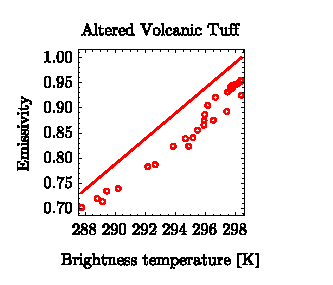
\includegraphics[scale=1]{pics/Chapter_03/AlteredVolcanicTuff_Emiss2BrightTemp.eps}
		\caption{}
	\end{subfigure}
	\vspace{1.5 em}
	\caption{Symbols represents examples of the relationship between brightness temperature $T_\mathrm{b}$ and emissivity as would be observed by TASI sensor. Lines illustrate the approximations of the relationship between brightness temperature and emissivity. The procedure used for estimation of the brightness temperature and emissivity relationship is described in text.}
\label{fig:relationship}
\end{figure}

The whole process of determining $\varepsilon_\mathrm{min}$ can be understood as smoothing the spectrum by finding the optimal value of $\varepsilon_\mathrm{min}$. Pseudocode depicted in Figure \ref{fig:FunctionCode} summarizes the above described procedure as a function \textsc{SmoothingErr}($\varepsilon_\mathrm{min},L_\mathrm{LL},L^\downarrow$) evaluating the error between Planck's law and estimated spectral radiance. This function is minimized with respect to the variable $\varepsilon_\mathrm{min}$ as follows:
\begin{equation*}
\underset{\varepsilon_\mathrm{min} \in  {[0.6,1]}}{\text{arg\,min}}\:\text{\textsc{SmoothingErr}}(\varepsilon_\mathrm{min},L_\mathrm{LL},L^\downarrow).
\label{eq:costFunction}
\end{equation*}

Continuous curves in Figure \ref{fig:relationship} show the optimal brightness temperature and emissivity relationship approximation. Let us emphasize that by applying emissivities obtained from the approximated relationship between brightness temperature and emissivity to (\ref{eq:lprime}), one gets $L^\prime$ as the best fit to Planck's law. This means that $B^{-1}(L^\prime_i)$ produces a temperature value for each band. These temperatures have minimum variability since they are derived from the best fit to Planck's law. Let us also remind the reader that maximum brightness temperature is coupled with emissivity equal to 1, which implies that it is part of the set of temperatures with smallest variability. It is important to note that maximum brightness temperature $T_\mathrm{b}$ computed from land-leaving radiance is usually smaller than surface temperature $T$ computed from surface radiance. Land-leaving radiance is smaller than surface radiance since natural materials are of emissivity higher than $0.6$ and the contribution from reflected downwelling radiance is usually much lower than surface radiance. By reason of maximum brightness temperature $T_\mathrm{b}$ being smaller than surface temperature $T$ and by being part of the set of temperatures with smallest variability, it can be concluded that maximum temperature from the set of temperatures tends to be the closest to the surface temperature $T$ and is therefore taken as the reference one.

\begin{figure}[!t]
\centering

\includegraphics[scale=1]{pics/Chapter_03/pseudo_code.pdf}
\vspace{1.5 em}
\caption{Pseudocode of the function that is being minimized in order to estimate the value of $\varepsilon_\mathrm{min}$.}
\label{fig:FunctionCode}
\end{figure}

Before passing emissivity to the Ratio and MMD modules, it is  {recomputed} according to the following equation:
\begin{equation}
\varepsilon_{ {i}} = \frac{L_{\mathrm{LL}_{ {i}}} - L^\downarrow_{ {i}}}{B_{ {i}}(T) - L^\downarrow_{ {i}}},
\label{eq:emissivityComputation}
\end{equation}
where $T$ is the maximum temperature associated with optimal $\varepsilon_\mathrm{min}$. Equation (\ref{eq:emissivityComputation}) is derived from (\ref{eq:landleavingRadiance}) and it is important for relating temperature and emissivity. This recomputation keeps temperature and emissivity consistent with each other (i.e. the same temperature can be derived from any emissivity band). The emissivity is then further processed with the Ratio and MMD modules, with minor changes to  {the} original version of the TES algorithm as it is described in \cite{GR99} and \cite{GR98}. These changes include: 1) there is no refinement of $\varepsilon_\mathrm{max}$ according to the emissivity spectral contrast, 2) the threshold $T_1$ for separation emissivities with small spectral contrast is not applied, and 3) the number of MMD iterations is set to one. Let us emphasize that before reporting algorithm outputs, emissivity is recomputed by (\ref{eq:emissivityComputation}) using the final value of temperature.





